\section{Practicality of VRF-based mining}
\label{sec:practicality}

In this section, we benchmark VRFs and compare their performance with existing hash functions for mining.
The experimental results show that VRF-based mining is easy to implement and introduces negligible overhead compared to hash-based mining.

\subsection{Experimental setting}

We implement the standardised EC-VRF in Algorithm~\ref{algo:standard-ecvrf} using Go programming language, without any optimisation.
We use Ed25519~\cite{bernstein2012high} as the underlying elliptic curve, Elligator~\cite{bernstein2013elligator} as $H_1(\cdot)$, SHA-3 as the hash function.
Ed25519, SHA-3 and the encoding of points on Ed25519 are supported by Go's standard library.
We use open-source implementations of SHA256D~\footnote{\url{https://github.com/seehuhn/sha256d}}, Scrypt~\footnote{\url{https://github.com/elithrar/simple-scrypt}}, and CryptoNight~\footnote{\url{https://github.com/Equim-chan/cryptonight}}.
All experiments run on a MacBook Pro with a 2.2 GHz Intel Core i7 Processor and a 16 GB DDR4 RAM.
Each group of experiments consists of ten runs, and we take the average value of ten values as the result.

\begin{figure}[htbp]
    \centering
    \begin{subfigure}[]{0.45\textwidth}
        \centering
        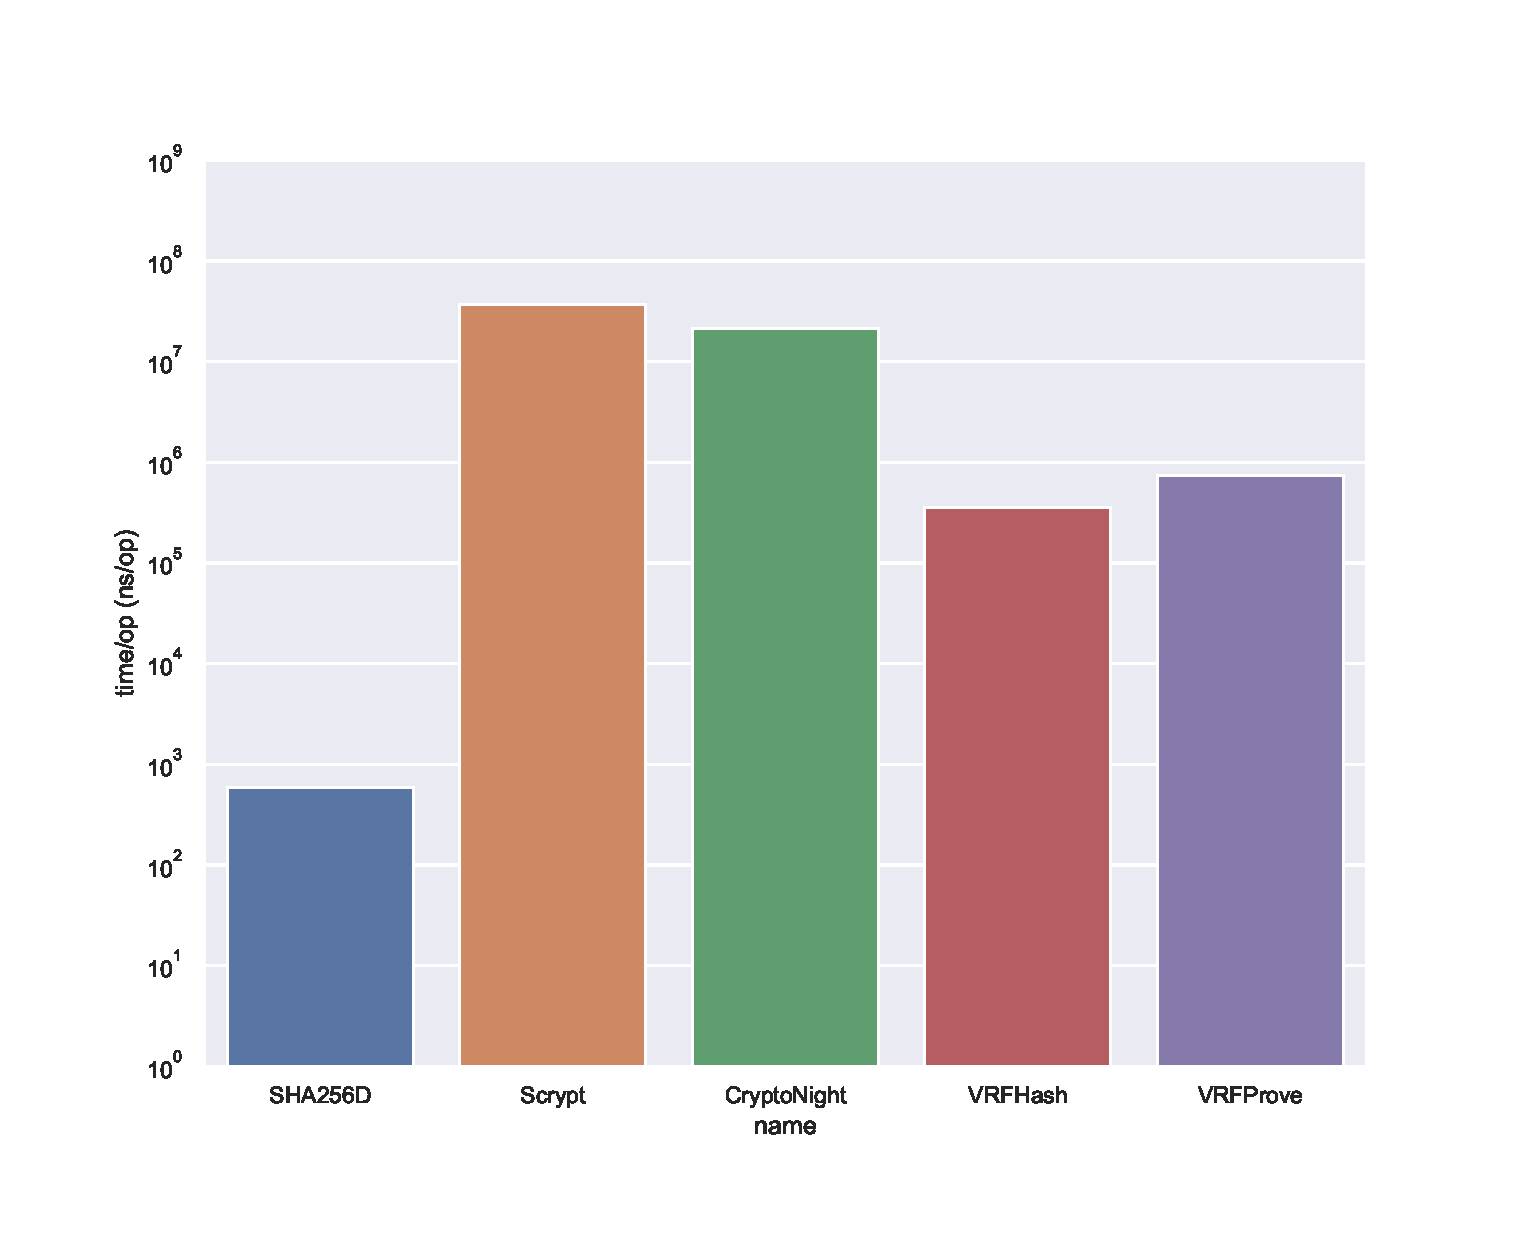
\includegraphics[width=\linewidth]{figs/runtime-comparison.eps}
        \caption{Comparing the runtime of VRF and other mining algorithms.}
        \label{fig:runtime-comparison}
    \end{subfigure}
    \hfill
    \begin{subfigure}[]{0.45\textwidth}
        \centering
        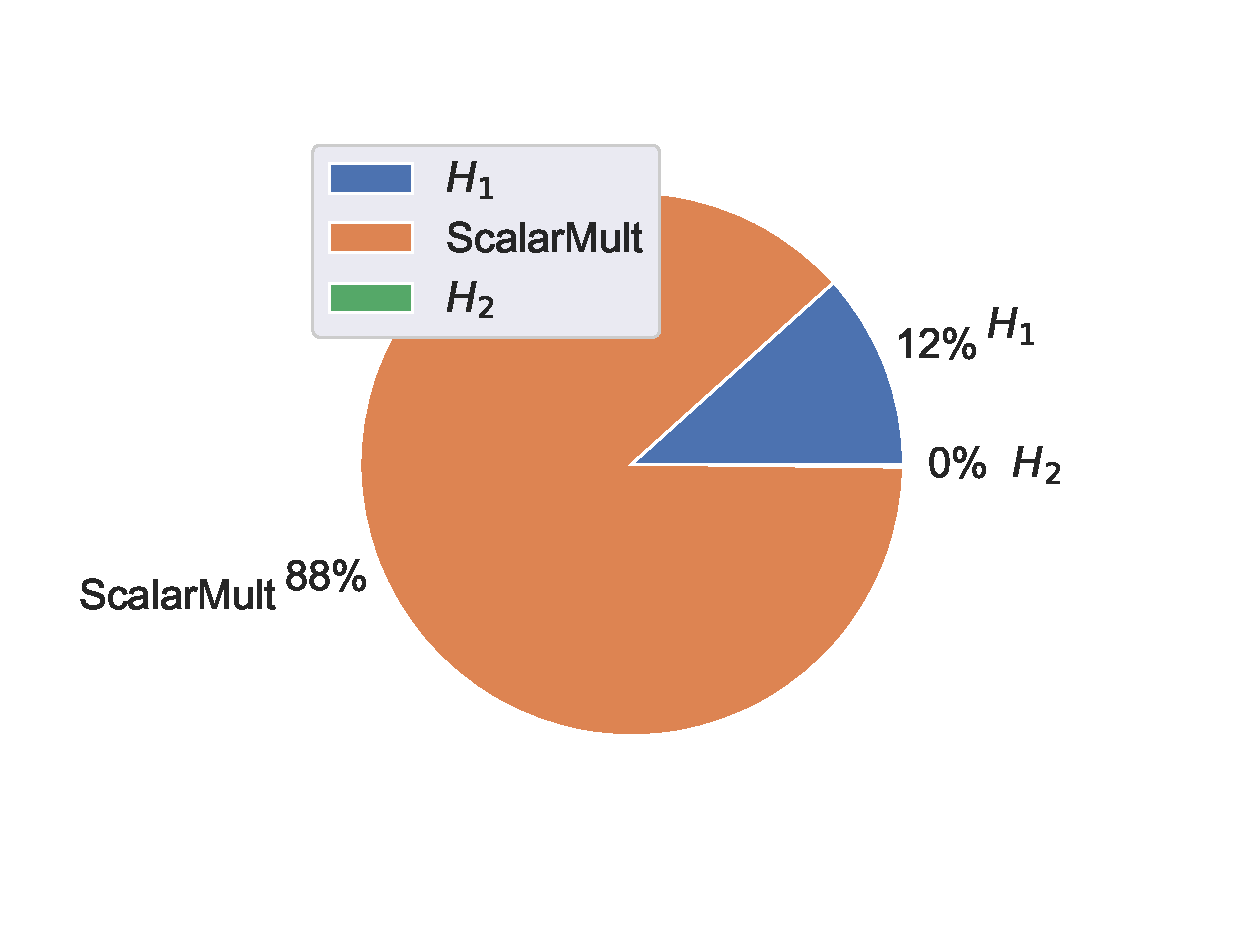
\includegraphics[width=\linewidth]{figs/runtime-breakdown.eps}
        \caption{Runtime breakdown of $\mathsf{VRFHash}(\cdot)$.}
        \label{fig:runtime-breakdown}
    \end{subfigure}
    \caption{Evaluation of VRF.}
\end{figure}

\subsection{VRF v.s. existing mining algorithms}

We compare the performance of VRF with existing mining algorithms.
Figure~\ref{fig:runtime-comparison} shows the runtime of VRF and other algorithms.
SHA256D is much faster than other algorithms, as SHA256D is simply executing SHA256 twice.
In addition, $\mathsf{VRFVerify}(\cdot)$ is slightly slower than $\mathsf{VRFProve}(\cdot)$, and $\mathsf{VRFProve}(\cdot)$ is slightly slower than $\mathsf{VRFHash}(\cdot)$.
Last, although without optimisation, all functions of VRF are much faster than Scrypt and CryptoNight.

\subsection{Runtime breakdown of VRF}

We profile $\mathsf{VRFHash}(\cdot)$ by evaluating its runtime of each step.
Figure~\ref{fig:runtime-breakdown} shows that, the elliptic curve scalar multiplication $\gamma \gets h^{sk}(\cdot)$ takes 88\% of $\mathsf{VRFHash}(\cdot)$'s running time.
This is because we use SHA-3 as the hash function in $H_1(\cdot)$ and $H_2(\cdot)$, and SHA-3 is designed to be fast.
Meanwhile, we calculate the elliptic curve scalar multiplication using the trivial double-and-add method without any optimisation, thus is much slower than $H_1(\cdot)$ and $H_2(\cdot)$.
There have been optimisation techniques for elliptic curve scalar multiplication, and some miners may exploit them for accelerating mining.
This may be unfair to other miners.
To avoid this, we suggest to replace $H_1(\cdot)$ and/or $H_2(\cdot)$ with slow hash functions such as Scrypt and CryptoNight.